% =====================================================================
% Projektna dokumentacija: Vizualizacija podataka — Eurosong
% Predmet: Vizualizacija podataka, FERIT Osijek
% =====================================================================

\documentclass[a4paper,11pt]{article}

% --- Encoding & jezik ------------------------------------------------
\usepackage[utf8]{inputenc}
\usepackage[T1]{fontenc}
\usepackage[croatian]{babel}

% --- Tipografija i layout --------------------------------------------
\usepackage[margin=2.5cm]{geometry}
\usepackage{lmodern}
\usepackage{microtype}
\usepackage{parskip}
\usepackage{setspace}
\setstretch{1.15}

% --- Boje, veze i naslovi --------------------------------------------
\usepackage{xcolor}
\definecolor{linkblue}{HTML}{1D4ED8}
\definecolor{accentorange}{HTML}{EA580C}
\definecolor{codebg}{HTML}{F1EFEA}
\definecolor{mutedgray}{HTML}{5B6473}
\definecolor{rulegray}{HTML}{D5D2CC}

\usepackage[
  colorlinks=true,
  linkcolor=black,
  urlcolor=linkblue,
  citecolor=black,
  pdftitle={Vizualizacija podataka --- Eurosong},
  pdfauthor={Student},
]{hyperref}

\usepackage{titlesec}
\titleformat{\section}{\Large\bfseries}{\thesection}{0.8em}{}
\titleformat{\subsection}{\large\bfseries}{\thesubsection}{0.7em}{}
\titleformat{\subsubsection}{\normalsize\bfseries}{\thesubsubsection}{0.6em}{}
\titlespacing*{\section}{0pt}{1.5em}{0.8em}
\titlespacing*{\subsection}{0pt}{1.2em}{0.5em}

% --- Slike, tablice, listing -----------------------------------------
\usepackage{graphicx}
\graphicspath{{images/}}
\usepackage{float}
\usepackage{caption}
\captionsetup{font={small,it},labelfont=bf,textfont=it,labelsep=period}

\usepackage{booktabs}
\usepackage{array}
\renewcommand{\arraystretch}{1.25}

\usepackage{listings}
\lstdefinestyle{codeblock}{
  basicstyle=\ttfamily\footnotesize,
  backgroundcolor=\color{codebg},
  frame=single,
  framerule=0pt,
  framexleftmargin=8pt,
  framexrightmargin=8pt,
  framextopmargin=6pt,
  framexbottommargin=6pt,
  breaklines=true,
  breakatwhitespace=true,
  showstringspaces=false,
  keywordstyle=\color{accentorange}\bfseries,
  commentstyle=\color{mutedgray}\itshape,
  stringstyle=\color{linkblue},
  language=,
  literate=%
    {č}{{\v c}}1 {ć}{{\' c}}1 {š}{{\v s}}1 {đ}{{\dj}}1 {ž}{{\v z}}1
    {Č}{{\v C}}1 {Ć}{{\' C}}1 {Š}{{\v S}}1 {Đ}{{\DJ}}1 {Ž}{{\v Z}}1,
  xleftmargin=8pt,
  xrightmargin=8pt,
}
\lstset{style=codeblock}

% --- Lista, popisi --------------------------------------------------
\usepackage{enumitem}
\setlist[itemize]{leftmargin=*,topsep=4pt,itemsep=2pt}
\setlist[enumerate]{leftmargin=*,topsep=4pt,itemsep=2pt}

% --- Naslovi odjeljaka u stilu KV-a; svaki odjeljak na novoj stranici -
\newcommand{\kv}[2]{\clearpage\section{KV#1 --- #2}}

% =====================================================================

\begin{document}

% --- Naslovnica ------------------------------------------------------
\begin{titlepage}
\centering
\vspace*{2cm}

{\Large\bfseries SVEUČILIŠTE JOSIPA JURJA STROSSMAYERA U OSIJEKU\par}
\vspace{0.4cm}
{\large Fakultet elektrotehnike, računarstva i informacijskih tehnologija Osijek\par}

\vspace{3cm}
{\itshape Projektni zadatak iz predmeta\par}
\vspace{0.6cm}
{\Huge\bfseries VIZUALIZACIJA PODATAKA\par}

\vspace{3cm}
{\LARGE\bfseries Interaktivna vizualizacija rezultata\\Eurosonga 2016.–2023.\par}

\vfill
\begin{flushleft}
\hspace{2cm}\textbf{Student:} {[}Ime i prezime{]}\par
\hspace{2cm}\textbf{Studij:} {[}Studij{]}\par
\end{flushleft}

\vspace{2cm}
{\itshape U Osijeku, svibanj 2026.\par}
\end{titlepage}

% --- Sadržaj ---------------------------------------------------------
\tableofcontents

% =====================================================================
\kv{1}{Definiranje projektnog zadatka}

\subsection{Projektni zadatak}

\textbf{Naziv zadatka:} Interaktivna vizualizacija rezultata Eurosonga 2016.–2023.

\textbf{Opis problema:} Eurovizijski rezultati kroz godine stvaraju velike količine podataka — bodovi žirija i publike (televote), plasmani, redoslijed nastupa, pjesme, izvođači te popularnost (npr.\ broj pregleda na YouTubeu). Tablice tih podataka teško pružaju brz uvid u trendove, najuspješnije zemlje ili veze među pojedinim pokazateljima. Cilj je objediniti više perspektiva u jedinstvenu interaktivnu vizualizaciju koja omogućuje brzo istraživanje podataka.

\textbf{Opis zadatka:} Izraditi web-aplikaciju s četiri međusobno povezana prikaza (karta Europe, stupčasti dijagram, linijski dijagram i dijagram raspršenja) koji dijele zajedničko stanje. Korisnik može filtrirati raspon godina, mijenjati prikazanu metriku i označiti zemlje koje ga zanimaju, a odabir se istovremeno odražava na svim prikazima.

\textbf{Cilj projekta:}
\begin{itemize}
  \item omogućiti istovremeni pregled uspješnosti zemalja iz više perspektiva: geografske raspodjele, rang-ljestvice, vremenskog tijeka i korelacija
  \item dati uvid u modernu eru (od 2016.\ nadalje), u kojoj se bodovi dijele na glasove žirija i glasove publike (televote)
  \item osigurati da se projekt može besplatno objaviti kao statična stranica na servisu GitHub Pages (bez poslužiteljskog dijela)
  \item osigurati neovisnost o vanjskim servisima u radu — obrađene datoteke podataka pohranjene su izravno u repozitoriju
\end{itemize}

\textbf{Poveznica na git repozitorij projekta:} \url{https://github.com/<korisnik>/<ime-repoa>}

\subsection{Podatci}

Podatci se kombiniraju iz triju javnih izvora.

\textbf{Spijkervet/eurovision-dataset} (GitHub izdanje iz 2023.):
\begin{itemize}
  \item \texttt{contestants.csv}: jedan red po nastupu — plasman u finalu, plasman u polufinalu, ukupni bodovi, bodovi žirija i publike, izvođač, naziv pjesme, poveznica na YouTube i redoslijed nastupa
  \item pokriva sve godine Eurosonga; u projektu se koristi samo razdoblje od 2016.\ nadalje
  \item Izvor: \url{https://github.com/Spijkervet/eurovision-dataset}
\end{itemize}

\textbf{Broj pregleda na YouTubeu:}
\begin{itemize}
  \item za svaku poveznicu iz prethodnog izvora broj pregleda dohvaća se parsiranjem HTML sadržaja stranice (regularnim izrazom)
  \item vrijednost se zapisuje u konačnu datoteku \texttt{entries.json}, uz lokalnu predmemoriju da se isti video ne dohvaća dvaput
\end{itemize}

\textbf{leakyMirror/map-of-europe (TopoJSON):}
\begin{itemize}
  \item granice europskih zemalja u TopoJSON zapisu, s ISO Alpha-2 oznakama u polju \texttt{id}
  \item omogućuje izravno povezivanje s datotekom \texttt{entries.json} preko polja \texttt{countryCode}
  \item Izvor: \url{https://github.com/leakyMirror/map-of-europe}
\end{itemize}

\subsection{Obrada podataka}

Obrada je provedena lokalno (Node.js), izvan repozitorija; u njega je uključen samo gotov rezultat --- datoteka \texttt{public/data/entries.json}. Postupak obrade odvija se u sljedećim koracima:

\begin{enumerate}
  \item učitavanje sirove datoteke \texttt{contestants.csv} (funkcijom \texttt{csvParse} iz paketa \texttt{d3-dsv})
  \item filtriranje: zadržavaju se samo godine $\geq 2016$ (prije 2016.\ nije postojala podjela bodova na žiri i publiku)
  \item filtriranje: redovi bez polja \texttt{place\_final} \emph{i} \texttt{place\_sf} odbacuju se (povučeni nastupi)
  \item preslikavanje dvoslovne oznake zemlje (npr.\ ,,hr'') u ISO Alpha-3 (npr.\ ,,HRV'') pomoću statičke mape oznaka; postoji i pričuvno preslikavanje punog imena zemlje u oznaku jer pojedini redovi sadrže puno ime umjesto oznake
  \item normalizacija naziva zemalja na hrvatski (npr.\ ,,Croatia'' $\to$ ,,Hrvatska'')
  \item označavanje \texttt{qualified=true} ako postoji \texttt{place\_final}, odnosno \texttt{false} ako postoji samo \texttt{place\_sf} (polufinalist koji se nije plasirao)
  \item sortiranje i zapisivanje u \texttt{public/data/entries.json}
  \item zaseban prolaz dohvaća broj pregleda s YouTubea uz ograničenje od 800\,ms između zahtjeva i upisuje vrijednost u polje \texttt{youtubeViews}
\end{enumerate}

\noindent\textbf{Rezultati obrade:}

\begin{table}[H]
\centering
\small
\begin{tabular}{ll}
\toprule
\textbf{Pokazatelj} & \textbf{Vrijednost} \\
\midrule
Ukupno nastupa & 288 (181 finalist + 107 polufinalista) \\
Godine & 7 (2016.–2023., 2020.\ otkazana) \\
Različitih zemalja & 44 \\
Dohvaćenih YouTube pregleda & 276 (za 12 nije dohvaćeno) \\
Veličina \texttt{entries.json} & 83 kB \\
Veličina \texttt{europe.topo.json} & 192 kB \\
\bottomrule
\end{tabular}
\caption{Statistika obrađenog skupa podataka.}
\end{table}

\subsection{Relevantne vrste prikaza za korištene podatke}

Razmatrane su četiri komplementarne vrste prikaza, od kojih svaka pokriva različitu analitičku dimenziju:

\begin{itemize}
  \item \textbf{Karta Europe (choropleth)} --- geografska raspodjela (gdje se nalaze najuspješnije zemlje?)
  \item \textbf{Stupčasti dijagram (top N)} --- rangiranje (koje su najbolje zemlje prema odabranoj metrici?)
  \item \textbf{Linijski dijagram po godinama} --- vremenski tijek (kako se uspješnost zemlje mijenja kroz godine?)
  \item \textbf{Dijagram raspršenja} --- korelacijska analiza (postoji li veza između npr.\ bodova žirija i bodova publike?)
\end{itemize}

% =====================================================================
\kv{2}{Dizajn vizualizacije podataka}

\subsection{Pitanja na koja vizualizacija daje odgovor}

Vizualizacija je oblikovana tako da odgovori na nekoliko konkretnih pitanja o rezultatima Eurosonga u promatranom razdoblju:

\begin{itemize}
  \item Koje zemlje prevladavaju na Eurosongu u ovoj eri (od 2016.\ nadalje)?
  \item Kako se uspješnost pojedine zemlje mijenja kroz godine?
  \item Postoji li geografski uzorak u uspješnosti — iz kojih regija Europe dolaze najuspješnije zemlje?
  \item Koliko je glasanje žirija usklađeno s glasanjem publike (televote)?
  \item Postoji li veza između broja pregleda nastupa na YouTubeu i njegova konačnog plasmana?
  \item Koje godine pojedine zemlje nisu prošle u finale (DNQ), a koja im je bila najuspješnija?
\end{itemize}

\subsection{Skica vizualizacije podataka}

Raspored je organiziran u mreži 2$\times$2:

\begin{itemize}
  \item gornji lijevi: karta Europe (choropleth) --- boja zemlje ovisi o odabranoj metrici
  \item gornji desni: stupčasti dijagram s top 8 zemalja
  \item donji lijevi: linijski dijagram plasmana kroz godine za top 5 zemalja
  \item donji desni: dijagram raspršenja s prekidačem između dvaju načina (bodovi žirija naspram televotea / broj pregleda naspram plasmana)
\end{itemize}

Iznad mreže nalazi se kontrolna traka: odabir metrike, klizač za raspon godina i prostor s oznakama odabranih zemalja.

\begin{figure}[H]
  \centering
  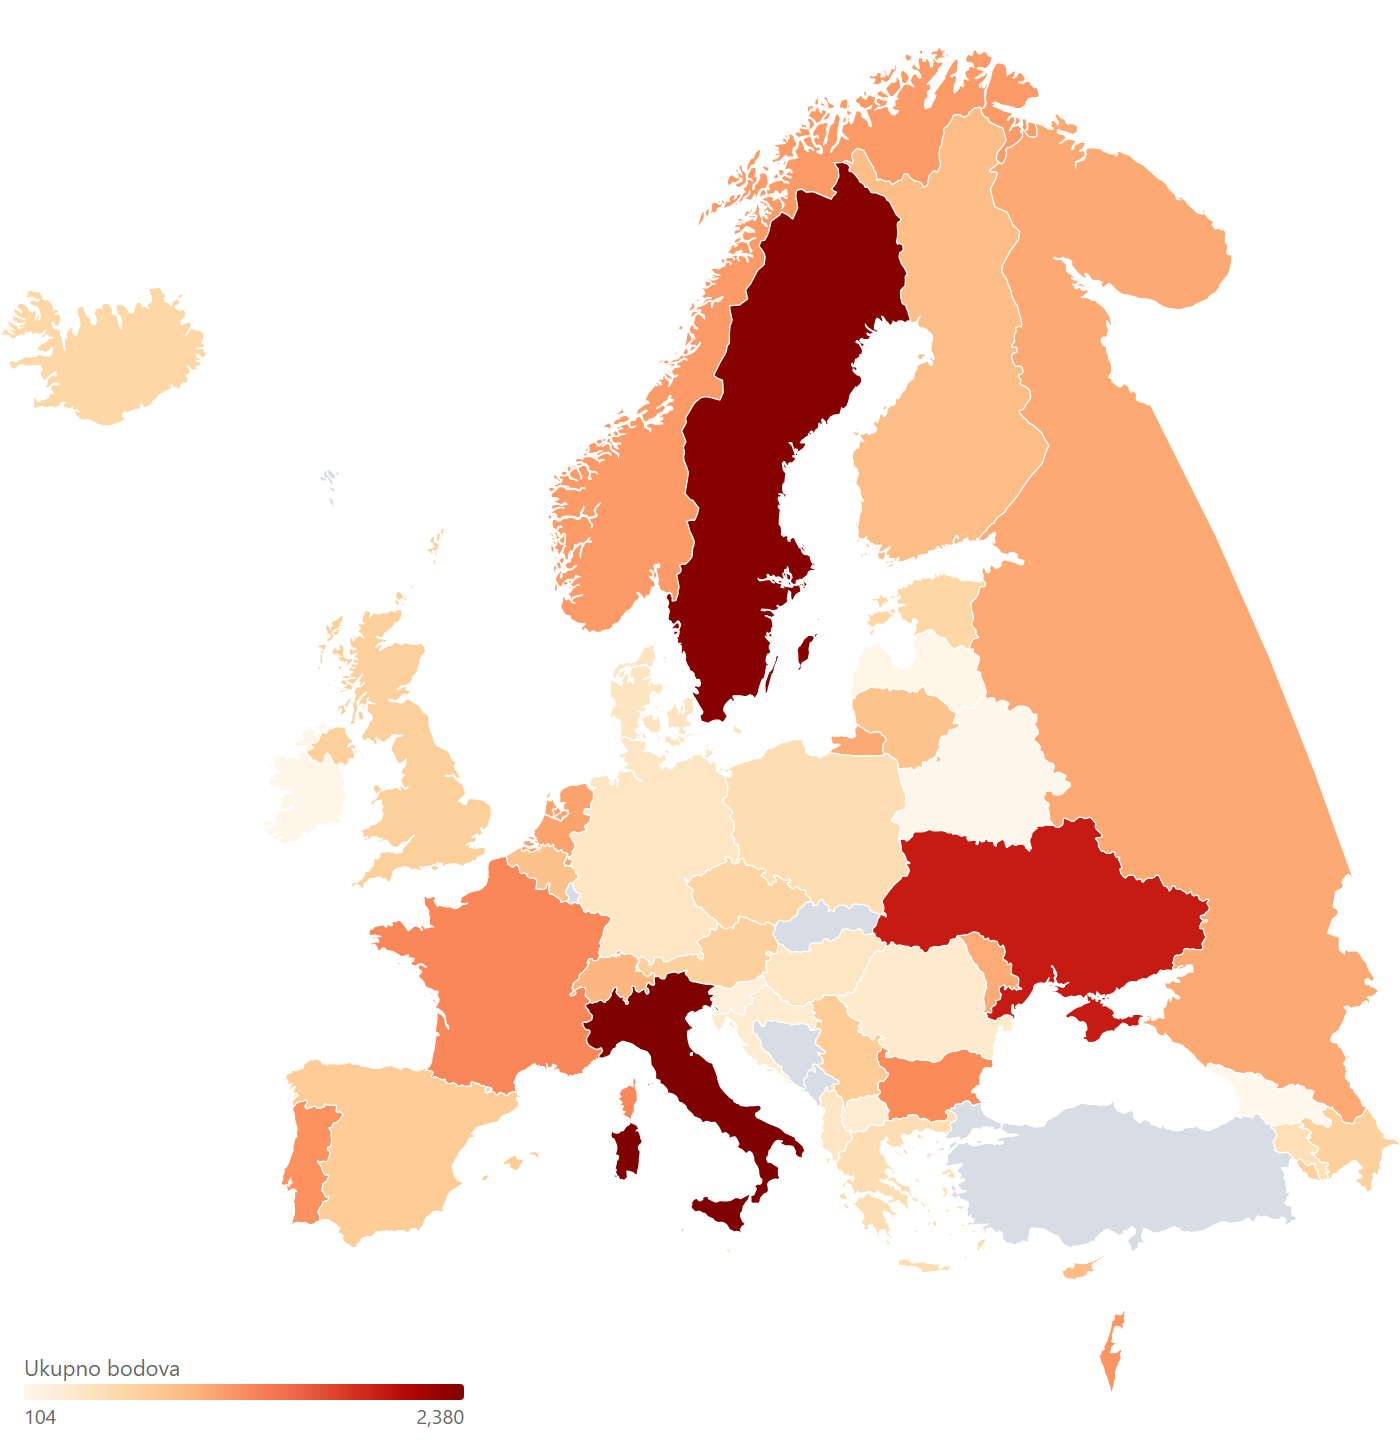
\includegraphics[width=0.85\textwidth]{map}
  \caption{Inicijalni izgled karte Europe --- choropleth po metrici ,,Ukupno bodova''.}
\end{figure}

\subsection{Postojeća rješenja i primjeri}

Slična rješenja koja su poslužila kao referenca tijekom dizajna:

\begin{itemize}
  \item zbirka primjera Observable D3 (\url{https://observablehq.com/@d3}) --- referenca za uobičajene D3 obrasce (skale, prijelazi, koordinatne osi)
  \item Bostockov primjer choropleth karte --- uzorak za geografsku projekciju i povezivanje podataka s oblicima
  \item galerija Datawrapper --- referenca za palete boja i urednu tipografiju
\end{itemize}

Konkretni dijelovi koda korišteni kao polazište:

\begin{itemize}
  \item \texttt{d3.geoMercator()}, \texttt{projection.fitSize()} i \texttt{d3.geoPath()} --- prema kodu iz priručnika kolegija (poglavlje Projekcije) za učitavanje TopoJSON zapisa, uklapanje karte u okvir i stvaranje SVG putanja
  \item \texttt{d3.scaleSequential(d3.interpolateOrRd)} --- standardni D3 obrazac za choropleth (promijenjen iz \texttt{interpolateYlOrRd} radi boljeg kontrasta na svijetloj pozadini)
  \item animacija crtanja linije pomoću svojstva \texttt{stroke-dashoffset} --- uobičajeni D3 idiom za ,,iscrtavanje'' linije
\end{itemize}

\subsection{Prilagodba podataka}

Sirova datoteka \texttt{contestants.csv} ($\sim$2,3 MB) prilagođena je u kompaktnu datoteku \texttt{entries.json} (83 kB). Izvorno sadrži 1734 reda s približno 20 stupaca, uključujući tekstove pjesama, poveznice i ostale stupce nepotrebne za vizualizaciju. Nakon obrade ostaje 288 redaka s 15 polja --- samo ono što se koristi.

Struktura jednog reda datoteke \texttt{entries.json}:

\begin{lstlisting}
{
  "year": 2016,
  "countryCode": "UA",
  "iso3": "UKR",
  "country": "Ukrajina",
  "performer": "Jamala",
  "song": "1944",
  "qualified": true,
  "place": 1,
  "placeSf": 2,
  "points": 534,
  "pointsJury": 211,
  "pointsTele": 323,
  "runningOrder": 21,
  "youtubeUrl": "https://youtube.com/watch?v=...",
  "youtubeViews": 33808082
}
\end{lstlisting}

Godina se referencira poljem \texttt{year} (broj), a zemlja poljem \texttt{countryCode} (ISO Alpha-2, velikim slovima). To omogućuje izravno povezivanje s TopoJSON zapisom koji koristi istu konvenciju.

\subsection{Boje i podatci}

\begin{table}[H]
\centering
\small
\begin{tabular}{p{3.5cm}p{4cm}p{6cm}}
\toprule
\textbf{Oznaka} & \textbf{Vrijednost} & \textbf{Korištenje} \\
\midrule
\texttt{--bg} & \#F7F6F3 (topli krem) & pozadina stranice \\
\texttt{--panel} & \#FFFFFF & kartice prikaza \\
\texttt{--accent} & \#EA580C (narančasta) & stupci, isticanje, glavna oznaka \\
\texttt{--accent-2} & \#1D4ED8 (plava) & označena zemlja na stupčastom dijagramu \\
\texttt{--text} & \#1C1917 & glavni tekst \\
\texttt{--muted} & \#6B6967 & osi, sekundarni tekst \\
\texttt{--no-data} & \#D8DDE5 & zemlje bez podataka na karti \\
\texttt{interpolateOrRd} & krem $\to$ tamnocrvena & gradijent choropleth karte \\
\texttt{schemeTableau10} & 10 osnovnih + dodatne & jedinstvena, stalna boja po zemlji \\
\bottomrule
\end{tabular}
\caption{Oznake boja i njihovo korištenje.}
\end{table}

Boje su odabrane prema trima prioritetima:

\begin{enumerate}
  \item vidljivost na svijetloj pozadini --- odbačena je hladna paleta i odabrana topla narančasta koja ima dobar kontrast s krem pozadinom
  \item raspoznatljivost --- najistaknutijih deset zemalja koristi perceptivno različite boje palete \texttt{schemeTableau10}, a ostale dobivaju dodatne razmaknute nijanse (po zlatnom kutu) tako da svaka zemlja ima jedinstvenu boju
  \item dosljednost --- ista boja zemlje koristi se u linijskom dijagramu, dijagramu raspršenja i oznakama (ne mijenja se pri promjeni filtra)
\end{enumerate}

% =====================================================================
\kv{3}{Izrada prototipne vizualizacije podataka}

\subsection{Osnovne funkcionalnosti i ponašanja}

Za prototip su identificirane sljedeće osnovne funkcionalnosti:

\begin{itemize}
  \item učitavanje podataka iz statičkih JSON datoteka u mapi \texttt{public/data/}
  \item iscrtavanje četiriju SVG prikaza u mreži 2$\times$2
  \item kontrolna traka: odabir metrike, dvostruki klizač za raspon godina, prostor s oznakama odabranih zemalja i gumb za poništavanje
  \item skočni opis (tooltip) pri prelasku pokazivačem --- prikazuje pojedinosti o zemlji ili nastupu
  \item klik na kartu, stupac ili točku --- uključuje ili isključuje odabir zemlje (moguće je odabrati više njih)
  \item prekidač ,,Samo odabrana zemlja'' iznad linijskog prikaza
  \item gumbi za prebacivanje između dvaju načina dijagrama raspršenja
\end{itemize}

Osnovna ponašanja proizlaze iz zajedničkog stanja: sva četiri prikaza dijele isto reaktivno stanje, pa se svaka promjena u kontrolnoj traci i svaki klik na zemlju u bilo kojem prikazu odmah odražavaju na ostalim prikazima. Klizači raspona godina zaštićeni su od preklapanja najmanjim razmakom od dvije godine, a stupčasti se dijagram pri promjeni preraspoređuje uz postupnu animaciju s kašnjenjem od 35\,ms po rednom broju stupca.

\subsection{Napredne funkcionalnosti i ponašanja}

Uz osnovne, predviđen je i niz naprednih funkcionalnosti koje omogućuju dublju analizu i precizniju interakciju:

\begin{itemize}
  \item odabir više zemalja istovremeno (oznake) --- svaka u svojoj boji
  \item ograničenje pokazivača --- kad je barem jedna zemlja označena, skočni opis prikazuje se samo nad njezinim točkama u linijskom dijagramu i dijagramu raspršenja
  \item stupčasti dijagram uključuje i označene zemlje izvan top 8 (dodaju se na dno, poredane po vrijednosti)
  \item linija se povlači i kroz godine bez plasmana u finalu (DNQ)
  \item poseban red ,,drugo'' na y-osi linijskog prikaza
  \item razlikovanje slučaja DNQ (ispala u polufinalu) i izostanka (nije sudjelovala) --- različiti skočni opisi
  \item invertirana skala stupaca za metrike kod kojih je manja vrijednost bolja --- kao referentna točka koristi se najgori mogući plasman (26)
  \item animirano crtanje linije pomoću svojstva \texttt{stroke-dashoffset}
\end{itemize}

\subsection{Implementacija osnovnih funkcionalnosti}

Glavna ulazna točka je \texttt{src/main.ts}, koja učitava podatke i stvara četiri prikaza:

\begin{lstlisting}
const [entries, topology] = await Promise.all([
  d3.json<Entry[]>(`${BASE_URL}data/entries.json`),
  d3.json<EuropeTopology>(`${BASE_URL}data/europe.topo.json`),
]);

const ctx = { entries, topology };
const chartList: ChartHandle[] = [
  createMap(document.getElementById("chart-map"), ctx),
  createBar(document.getElementById("chart-bar"), ctx),
  createLine(document.getElementById("chart-line"), ctx),
  createScatter(document.getElementById("chart-scatter"), ctx),
];

function renderAll(state) {
  for (const c of chartList) c.update(state);
}
subscribe((state) => renderAll(state));
\end{lstlisting}

Svaka funkcija za stvaranje prikaza vraća sučelje \texttt{\{ update(state) \}}. Promjena stanja poziva metodu \texttt{update} na svim prikazima, a svaki prikaz sam odlučuje što treba ponovno iscrtati.

\begin{figure}[H]
  \centering
  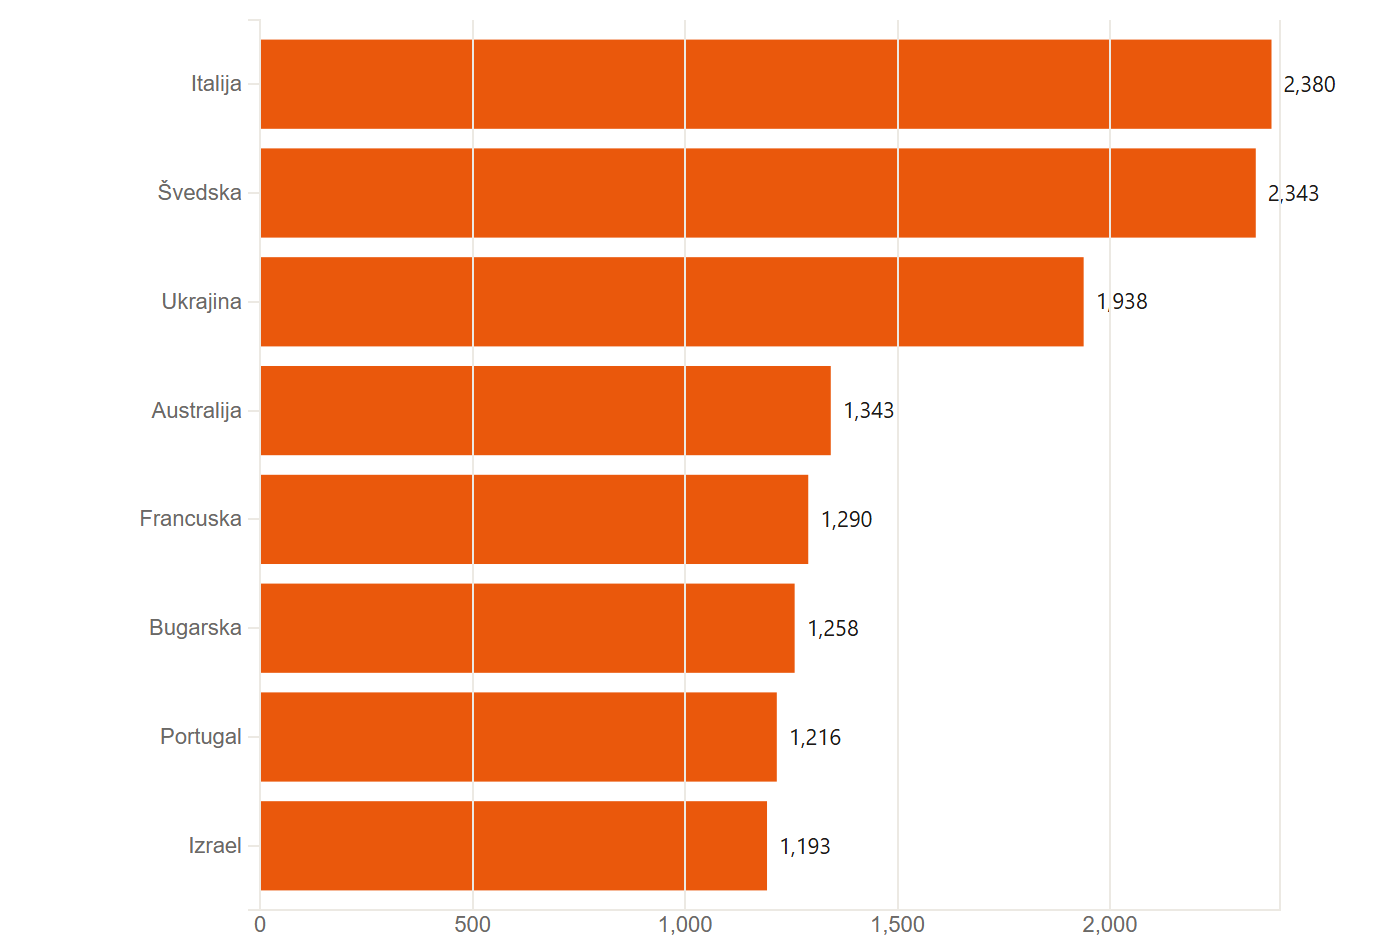
\includegraphics[width=0.85\textwidth]{bar}
  \caption{Stupčasti dijagram s top 8 zemalja po ukupnim bodovima.}
\end{figure}

\subsection{Implementacija osnovnog ponašanja}

Reaktivno stanje implementirano je u \texttt{src/state.ts} kao jednostavna pohrana s mehanizmom pretplate. Skup (\texttt{Set}) se ne smatra promijenjenim po referenci --- pri promjeni odabira uvijek se stvara novi skup:

\begin{lstlisting}
export function setState(patch: StatePatch): void {
  let changed = false;
  for (const k in patch) {
    const prev = state[k], next = patch[k];
    if (prev instanceof Set && next instanceof Set) {
      if (!setEq(prev, next)) { state[k] = next; changed = true; }
    } else if (prev !== next) { state[k] = next; changed = true; }
  }
  if (changed) for (const l of listeners) l(state, patch);
}

export function toggleSelected(code: string): Set<string> {
  const next = new Set(state.selectedCountries);
  if (next.has(code)) next.delete(code); else next.add(code);
  return next;
}
\end{lstlisting}

Klik na zemlju u bilo kojem prikazu poziva istu funkciju:

\begin{lstlisting}
setState({ selectedCountries: toggleSelected(d.countryCode) });
\end{lstlisting}

\begin{figure}[H]
  \centering
  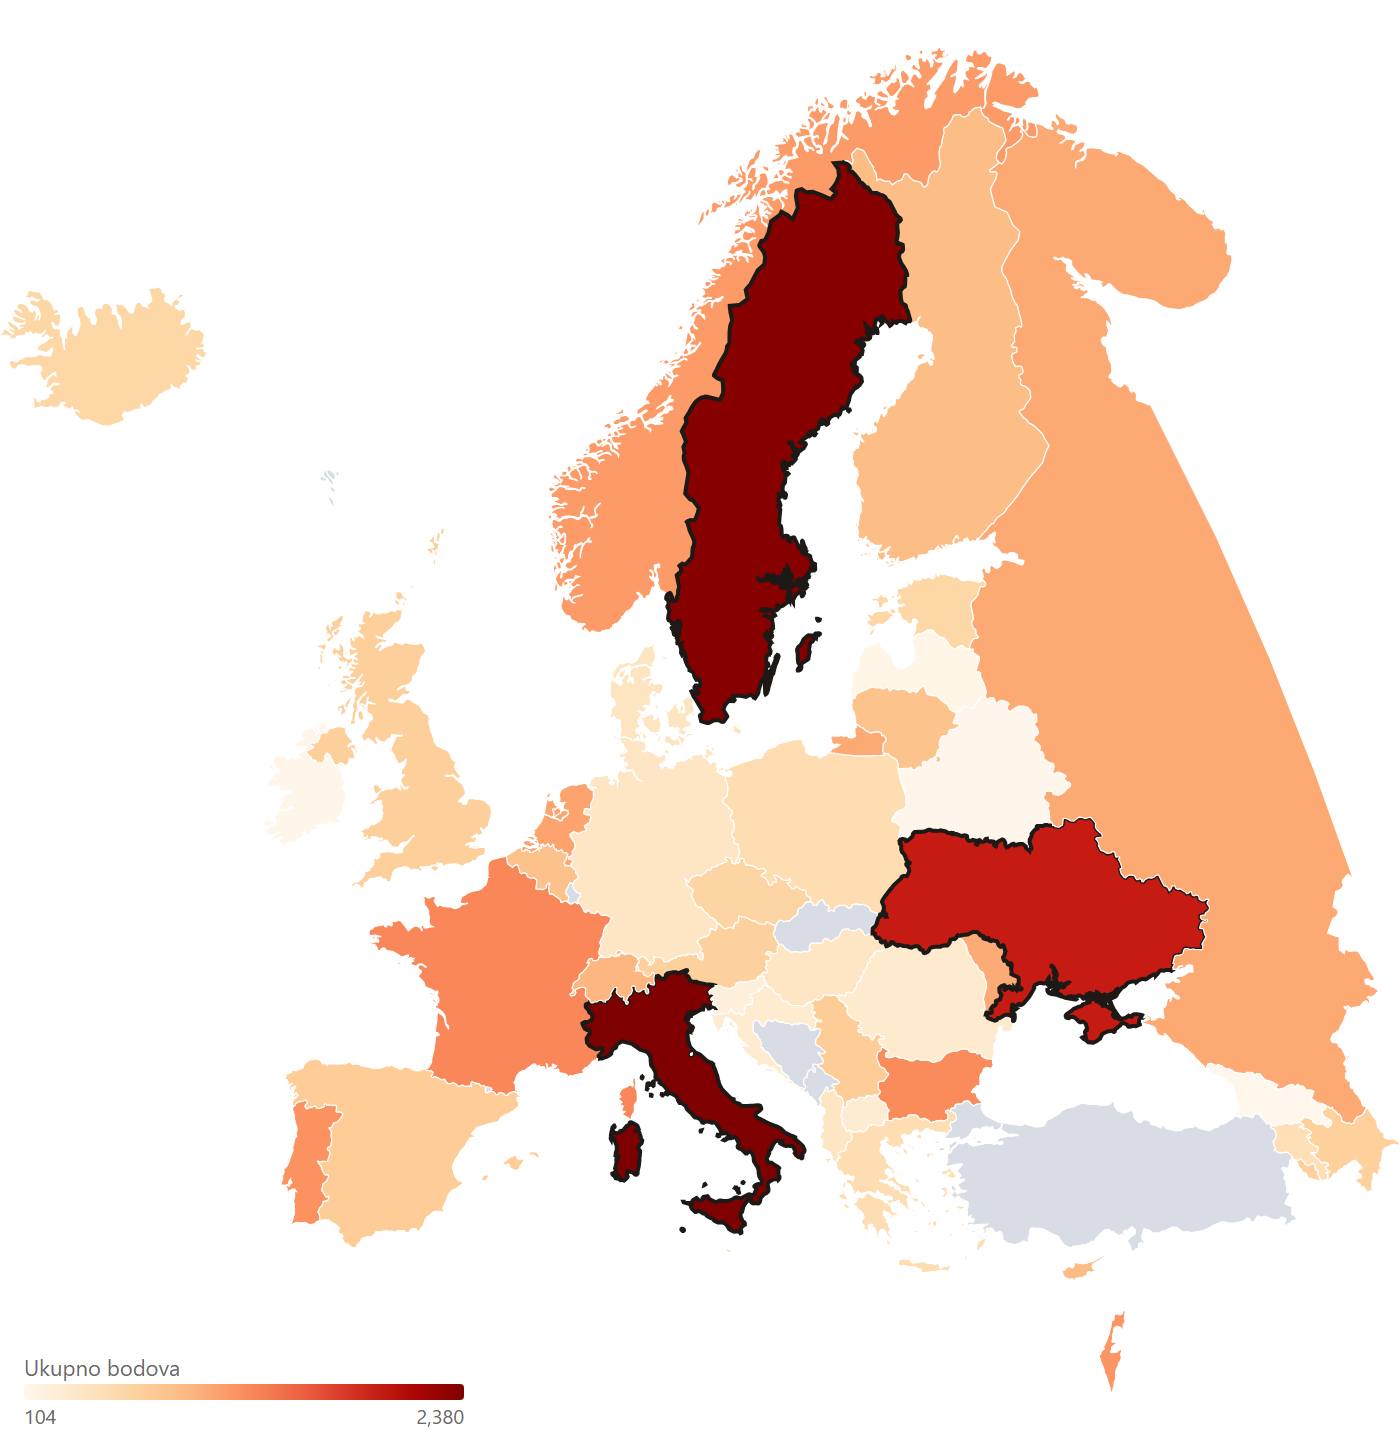
\includegraphics[width=0.85\textwidth]{map_selected}
  \caption{Karta s označenim zemljama --- odabrane imaju tamniji obrub.}
\end{figure}

% =====================================================================
\kv{4}{Izrada konačne vizualizacije podataka}

\subsection{Implementacija osnovnih funkcionalnosti}

U konačnoj su verziji dovršene sve osnovne funkcionalnosti te su uvedene tri dodatne dorade. Prikaz je prilagođen mobilnim uređajima: ispod 980\,px prelazi u jedan stupac, a na užim zaslonima (ispod 640\,px) klizač dobiva veći klizni element radi dodira (22\,px), dok kontrole zauzimaju punu širinu. Oba klizača raspona godina dijele isti raspon, a vrijednost se pri pomicanju ograničava tako da se klizni elementi ne mogu preklopiti i time čuva najmanji razmak od dvije godine. Naposljetku, označena zemlja koja nije u prikazanom skupu automatski se uključuje u stupčasti i linijski prikaz, dodana na dno.

\begin{figure}[H]
  \centering
  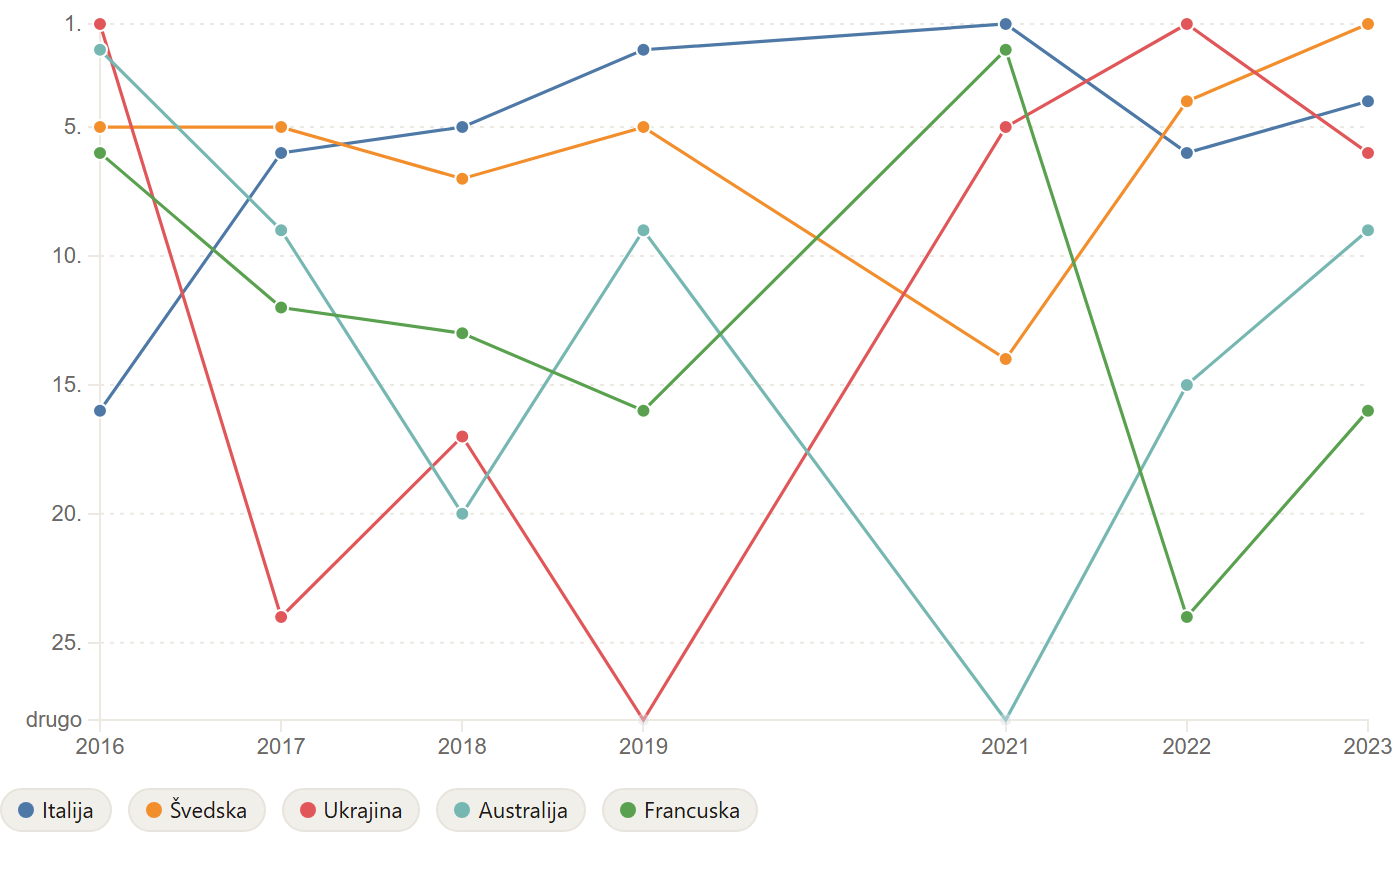
\includegraphics[width=0.85\textwidth]{line}
  \caption{Linijski dijagram --- plasmani top 5 zemalja kroz 2016.–2023. Sive točke označavaju godine bez plasmana u finalu (red ,,drugo'').}
\end{figure}

\subsection{Implementacija osnovnog ponašanja}

Središnja je zamisao da svi prikazi reagiraju isključivo na stanje. Promjena načina dijagrama raspršenja ne odvija se izravnim pozivom, nego promjenom stanja funkcijom \texttt{setState}:

\begin{lstlisting}
// main.ts -- rukovatelj klikom na gumb
tabs.forEach((t) => {
  t.addEventListener("click", () => {
    const mode = t.dataset.mode as ScatterMode;
    tabs.forEach((b) => b.classList.toggle("active", b === t));
    setState({ scatterMode: mode });
  });
});

// scatter.ts -- reagira na state.scatterMode
function update(state: AppState): void {
  cfg = resolveConfig(state.scatterMode);
  // ... iscrtavanje s novom konfiguracijom
}
\end{lstlisting}

Time se uklanja zaobilazna komunikacija preko globalnih varijabli i postiže jedinstveni izvor istine (engl.\ \emph{single source of truth}).

\subsection{Implementacija naprednih funkcionalnosti}

\subsubsection*{Poseban red ,,drugo'' u linijskom prikazu}

Y-skala se ne ograničava na \texttt{maxPlace} (do 26), nego se proširuje za \texttt{DNQ\_PAD} (dvije jedinice). Posebna vrijednost na osi, \texttt{dnqRow = maxPlace + 2}, prikazuje se oznakom ,,drugo'' umjesto broja. Točke za nastupe bez plasmana crtaju se na tom položaju, ostajući unutar grafa:

\begin{lstlisting}
const dnqRow = maxPlace + DNQ_PAD;
const y = d3.scaleLinear().domain([1, dnqRow]).range([0, innerH]);
const dnqY = y(dnqRow);

const yTickValues = [...stdTicks, dnqRow];
gYAxis.call(
  d3.axisLeft(y)
    .tickValues(yTickValues)
    .tickFormat((d) => (+d === dnqRow ? "drugo" : `${d}.`))
);
\end{lstlisting}

\subsubsection*{Invertirana skala stupaca za metrike kod kojih je manja vrijednost bolja}

Za metriku ,,Prosječni plasman'', kod koje je manja vrijednost bolja, izravan pristup \texttt{x(value)} dao bi kratke stupce za dobre zemlje. Rješenje je kao referentnu točku koristiti \texttt{scaleMax} (26, najgori mogući plasman), pa je širina jednaka \texttt{x(scaleMax - value)}. Tako Rusija s prosječnim plasmanom 5,0 dobiva širinu od 51\,px, a Azerbajdžan s 15,0 dobiva 27\,px (omjer 1,89:1 umjesto nerazmjernih $\sim$250:1 kod naivnog pristupa).

\begin{lstlisting}
const refMax = metric.scaleMax ?? xMax;
const x = metric.higherIsBetter
  ? d3.scaleLinear().domain([0, xMax]).nice().range([0, innerW])
  : d3.scaleLinear().domain([0, refMax]).range([0, innerW]);
const barLen = (v) =>
  metric.higherIsBetter ? x(v) : Math.max(2, x(refMax - v));
\end{lstlisting}

\subsubsection*{Prebacivanje načina dijagrama raspršenja}

Dijagram raspršenja ima dva načina: bodovi žirija naspram bodova publike (linearne osi) te broj pregleda naspram plasmana (logaritamska x-os, invertirana y-os). Konfiguracija \texttt{MODES} definirana je unutar \texttt{scatter.ts}:

\begin{lstlisting}
const MODES: Record<ScatterMode, ScatterConfig> = {
  jt: {
    xKey: "pointsJury", yKey: "pointsTele",
    xLabel: "Bodovi žirija", yLabel: "Bodovi televotea",
  },
  yt: {
    xKey: "youtubeViews", yKey: "place",
    xLabel: "YouTube pregledi", yLabel: "Plasman u finalu",
    xLog: true, yInvert: true,
  },
};
\end{lstlisting}

\begin{figure}[H]
  \centering
  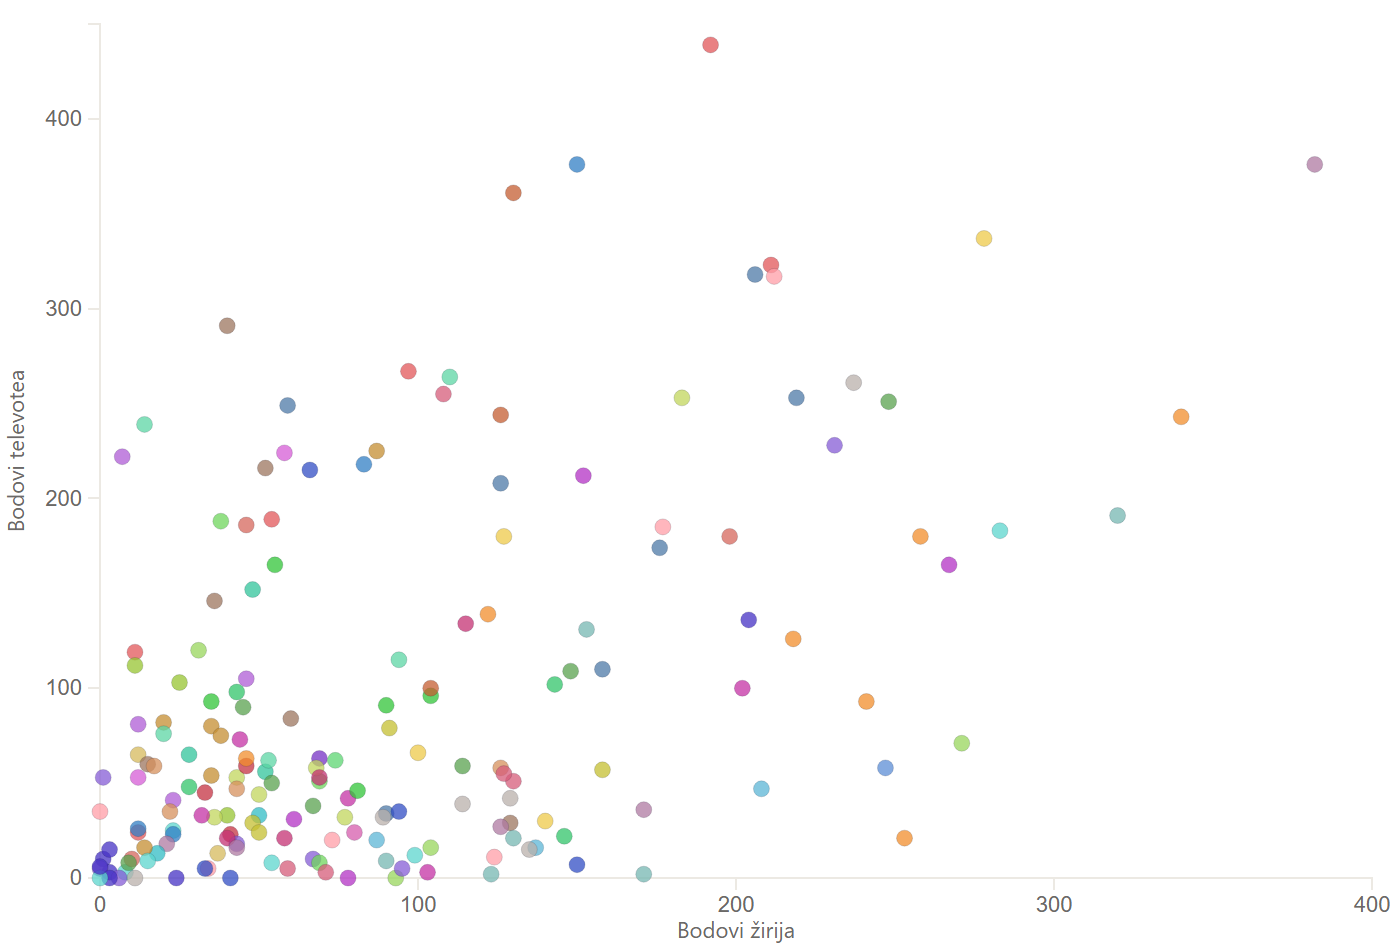
\includegraphics[width=0.85\textwidth]{scatter}
  \caption{Dijagram raspršenja --- bodovi žirija (x) naspram bodova publike (y) za sve finaliste 2016.–2023.}
\end{figure}

\subsection{Implementacija naprednog ponašanja}

\subsubsection*{Animirano crtanje linija}

Kada se linija prvi put pojavi u prikazu --- kad zemlja uđe u prikazani skup (npr.\ nakon promjene metrike ili raspona godina) ili kad je korisnik označi izvan trenutnog prikaza --- iscrtava se slijeva nadesno; već prikazane linije ostaju na mjestu i ne animiraju se ponovno. Točke se prve postave (\texttt{POINT\_REVEAL\_MS} = 380\,ms), a zatim uz odgodu kreće animacija svojstva \texttt{stroke-dashoffset} (\texttt{LINE\_DELAY\_MS} = 320\,ms, \texttt{LINE\_DRAW\_MS} = 1300\,ms). Poziv \texttt{interrupt()} prekida tekuću animaciju ako se prikaz osvježi prebrzo:

\begin{lstlisting}
allLines.each(function () {
  const len = this.getTotalLength();
  const sel = d3.select(this);
  sel
    .interrupt("line-draw")
    .attr("stroke-dasharray", `${len} ${len}`)
    .attr("stroke-dashoffset", len)
    .transition("line-draw")
    .delay(LINE_DELAY_MS)
    .duration(LINE_DRAW_MS)
    .ease(d3.easeCubicOut)
    .attr("stroke-dashoffset", 0);
});
\end{lstlisting}

\subsubsection*{Ograničenje pokazivača na označene zemlje}

Kad je barem jedna zemlja označena, neoznačene točke u linijskom prikazu i dijagramu raspršenja postaju neinteraktivne (\texttt{pointer-events: none}) i prigušene. Time se za prikaz pojedinosti izdvajaju samo relevantne točke:

\begin{lstlisting}
.style("pointer-events", (d) =>
  hasSelection && !state.selectedCountries.has(d.e.countryCode)
    ? "none" : "auto",
);
\end{lstlisting}

\begin{figure}[H]
  \centering
  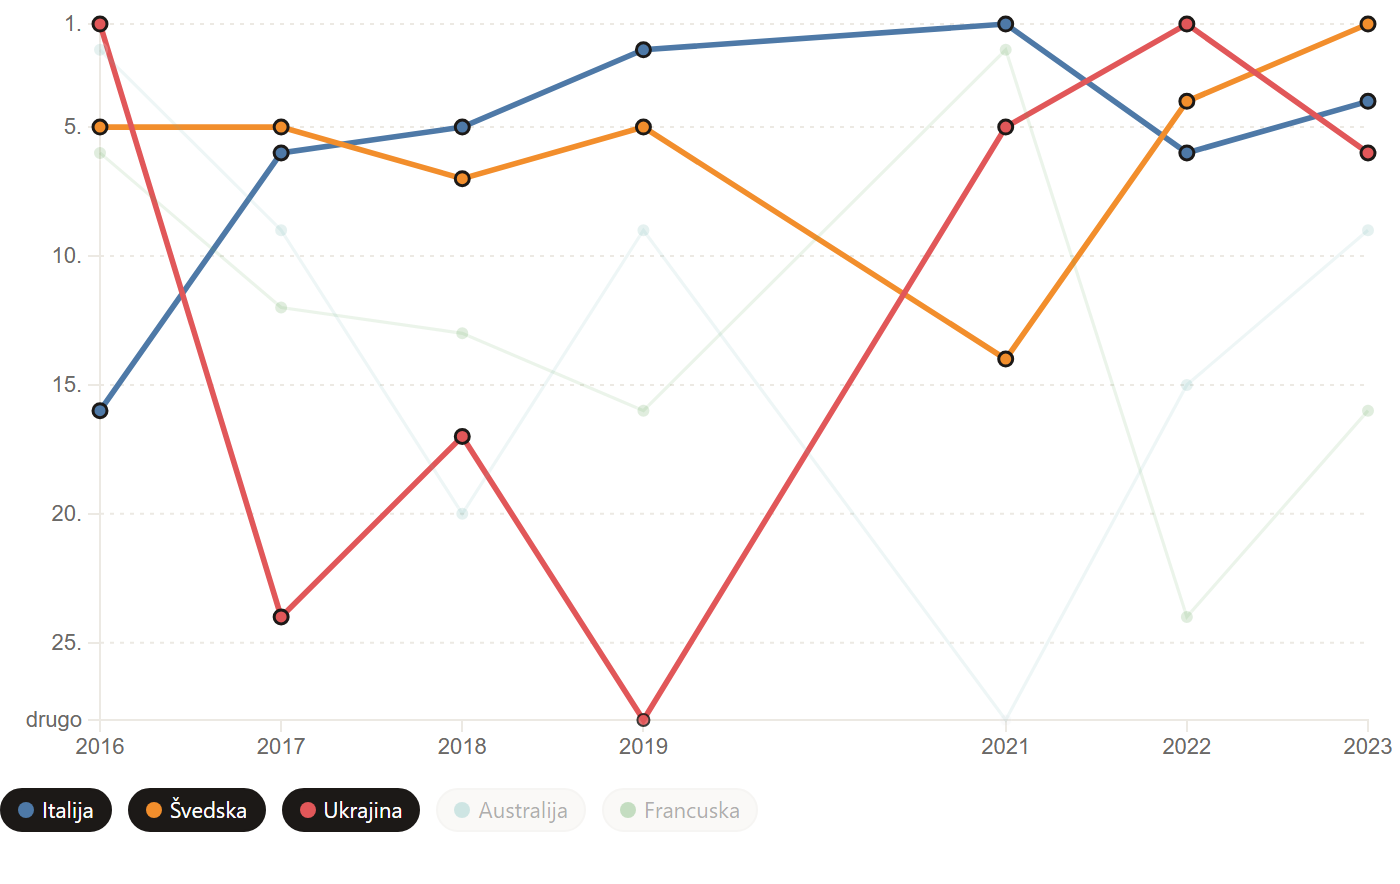
\includegraphics[width=0.85\textwidth]{line_selected}
  \caption{Linijski prikaz s označenim zemljama --- ostale su linije prigušene, a pokazivač ograničen.}
\end{figure}

% =====================================================================
\kv{5}{Dovršetak projektnog zadatka i pisanje dokumentacije}

\subsection{Eventualne preinake i dorade rješenja}

Tijekom završne faze projekta napravljene su sljedeće preinake:

\begin{itemize}
  \item prelazak na TypeScript --- sve datoteke u \texttt{src/} prevedene su iz \texttt{.js} u \texttt{.ts} uz domenske tipove (\texttt{Entry}, \texttt{AppState}, \texttt{MetricKey}, \texttt{AggregateMetric} i dr.)
  \item preoblikovanje načina dijagrama raspršenja na model vođen stanjem --- uklonjena je globalna varijabla \texttt{window.\_\_setScatterMode}, a jedinstveni izvor istine postaje \texttt{state.scatterMode}
  \item čišćenje stanja --- uklonjena su neiskorištena polja iz ranije inačice s približavanjem karte
  \item ujednačavanje stila koda --- dosljedno formatiranje i imenovanja kroz sve module
  \item potpuna neovisnost o vanjskim servisima u radu --- svi su podatci unaprijed obrađeni i pohranjeni kao statične JSON datoteke u \texttt{public/data/}, pa aplikacija radi i bez internetske veze
  \item dodavanje favikona (SVG) i meta-opisa za karticu preglednika i pretpregled pri dijeljenju
  \item dodavanje pristupačnih oznaka (\texttt{role="img"}, \texttt{aria-label}) na sve SVG prikaze radi podrške čitačima zaslona
  \item dodavanje JSDoc komentara na ključne izvezene funkcije
\end{itemize}

\subsection{Izrada projektne dokumentacije}

\subsubsection*{Hijerarhija projekta}

\begin{lstlisting}
github-projekt/
|-- index.html                 glavni HTML
|-- vite.config.js             Vite konfiguracija
|-- tsconfig.json              TypeScript konfiguracija
|-- package.json
|-- README.md
|-- public/
|   |-- favicon.svg
|   `-- data/                  staticki JSON-i koje stranica ucitava
|       |-- entries.json       288 nastupa s brojem pregleda
|       `-- europe.topo.json   TopoJSON Europe
|-- src/
|   |-- main.ts                ulazna tocka + kontrole
|   |-- state.ts               reaktivno stanje
|   |-- types.ts               domenski tipovi
|   |-- metrics.ts             definicije metrika + agregacije
|   |-- tooltip.ts             skocni opis
|   |-- colors.ts              stalna paleta boja po zemlji
|   |-- styles.css
|   `-- charts/
|       |-- map.ts             choropleth karta
|       |-- bar.ts             stupcasti dijagram (top 8)
|       |-- line.ts            linijski dijagram (red "drugo")
|       `-- scatter.ts         dijagram rasprsenja (2 nacina)
`-- .github/workflows/
    `-- deploy.yml             automatska objava na GitHub Pages
\end{lstlisting}

Napomena: skripte za pripremu podataka (\texttt{scripts/}) ne nalaze se u repozitoriju jer ih vizualizacija ne treba u radu --- obrađeni podatci već su pohranjeni u \texttt{public/data/}.

\subsubsection*{Popis korištenih tehnologija}

\begin{itemize}
  \item D3.js v7
  \item TopoJSON
  \item TypeScript
  \item Vite
  \item Node.js
  \item GitHub Actions
  \item GitHub Pages
\end{itemize}

\subsubsection*{Upute za postavljanje}

\begin{lstlisting}
# 1. Kloniraj repozitorij
git clone https://github.com/<korisnik>/<ime-repoa>.git
cd <ime-repoa>

# 2. Instaliraj ovisnosti
npm install

# 3. Pokreni razvojni posluzitelj
npm run dev          # http://localhost:5173
\end{lstlisting}

Za produkcijsku izradu:

\begin{lstlisting}
npm run build        # rezultat u dist/
npm run preview      # lokalni pregled produkcijske izrade
\end{lstlisting}

\textbf{Objava na GitHub Pages:}

\begin{enumerate}
  \item postaviti repozitorij na GitHub
  \item Settings $\to$ Pages $\to$ Source: GitHub Actions
  \item nakon svakog pusha na granu \texttt{main} radni tok u \texttt{.github/workflows/deploy.yml} automatski izrađuje i objavljuje stranicu
\end{enumerate}

\subsubsection*{Upute za korištenje}

\textbf{Kontrolna traka (gornji dio):}

\begin{itemize}
  \item Metrika --- odabire se metrika koja se primjenjuje na kartu i stupčasti dijagram
  \item Raspon godina --- povlačenjem klizača sužava se raspon; najmanji razmak je dvije godine (npr.\ 2016.–2018.)
  \item Označene zemlje --- prikazuju se kao oznake nakon klika na zemlju; gumb ,,$\times$'' uklanja oznaku
  \item Poništavanje --- vraća sve filtre na početne vrijednosti
\end{itemize}

\textbf{Interakcije unutar prikaza:}

\begin{itemize}
  \item Karta --- klik na zemlju s podatcima uključuje ili isključuje njezino označavanje; prelaskom pokazivača prikazuje se skočni opis
  \item Stupčasti dijagram --- klik na stupac ili oznaku zemlje uključuje ili isključuje odabir; označene zemlje izvan top 8 dodaju se na dno
  \item Linijski dijagram --- prelazak pokazivačem nad točkom prikazuje pjesmu i izvođača; klik na oznaku iznad grafa uključuje ili isključuje zemlju
  \item Dijagram raspršenja --- gumbi (gore desno) prebacuju između načina ,,Žiri vs televote'' i ,,YouTube vs plasman''
\end{itemize}

% =====================================================================
\clearpage
\section*{Literatura}
\addcontentsline{toc}{section}{Literatura}

\begin{enumerate}
  \item Spijkervet, J.\ (2023). \emph{Eurovision Dataset}. GitHub izdanje. \\\url{https://github.com/Spijkervet/eurovision-dataset}
  \item leakyMirror.\ (2018). \emph{Map of Europe TopoJSON}. \\\url{https://github.com/leakyMirror/map-of-europe}
  \item Bostock, M.\ (2017). \emph{D3.js --- Data-Driven Documents (v7)}. \url{https://d3js.org/}
  \item Job, J., Livada, Č.\ (2016). \emph{Vizualizacija podataka --- priručnik za laboratorijske vježbe}. FERIT Osijek.
  \item \emph{Vite --- alat za izradu web-aplikacija}. \url{https://vitejs.dev/}
  \item \emph{TypeScript}. \url{https://www.typescriptlang.org/}
\end{enumerate}

% =====================================================================
\clearpage
\section*{Prilog I}
\addcontentsline{toc}{section}{Prilog I}

\textbf{Poveznica na git repozitorij projekta:} \url{https://github.com/<korisnik>/<ime-repoa>}

Cjelovit programski kod (TypeScript, $\sim$2600 redaka) dostupan je u javnom GitHub repozitoriju. Organizacija koda po modulima i uloga svake pojedine datoteke prikazani su ranije, u prikazu hijerarhije projekta (poglavlje KV5).

\end{document}
